\documentclass[../DISSERTACAO_MAIN.tex]{subfiles}

\begin{document}
	
\section{Montagem e anotação dos mitogenomas de \textit{Pseudomyrmecinae}}
	
	Os 14 conjuntos de dados genômicos usados para montar o mitogenoma completo das formigas pertencentes à subfamília Pseudomirmecinae foram baixados do banco de dados SRA (Tabela \ref{tab:datasets}). Dois tipos de datasets diferentes foram usados: (i) Sequenciamento do Genoma Completo (WGS), que frequentemente continha uma quantidade maior de dados de sequenciamento, totalizando 212,7 Giga pares de base (Gpb) para seis espécies (de acordo com a informação fornecida pelo SRA); uma média de 35,45 Gpb por espécie (Rubin \& Moreau, 2016); e (ii) experimentos de UCE, para os quais realizamos o download  de 5,94 Gpb para oito espécies; uma média de 742,5 Mpb por espécie (Branstetter et al., 2017; Ward \& Branstetter, 2017).
	
	O dataset completo baixado para cada espécie foi usado como entrada para uma montagem de novo usando o montador NOVOPlasty. Após essa primeira etapa de montagem do genoma, usamos um subconjunto contendo dois ou quatro milhões de reads de sequenciamento como entrada para uma segunda etapa de montagem do genoma usando o software MIRA. Este procedimento foi realizado para mapear as reads na montagem preliminar e melhorar a qualidade do mitogenoma. Para alguns mitogenomas, o MIRA não conseguiu produzir o genoma mitocondrial completo e circularizado. Nesse caso, uma terceira etapa de montagem foi necessária, na qual o maior contig gerado pelo MIRA foi usado como backbone para concluir a montagem usando o MITObim (Tabela \ref{tab:montagem}). Esta metodologia foi capaz de montar a mitocôndria completa de todas as espécies de Pseudomyrmecinae analisadas, com exceção da T. aethiops, para a qual tivemos que usar o dataset completo como entrada para MIRA e MITObim ao invés de filtrar o subconjunto de reads na segunda etapa. O uso de múltiplas estratégias para montar as sequências mitocondriais completas era esperado, já que dados de NGS são variáveis entre diferente espécies e corridas de sequenciamento. Além disso, os datasets usados aqui vieram de trabalhos com abordagens experimentais diferentes, o que provavelmente potencializou a variabilidade de conjuntos de dados já muito díspares entre si. Os 14 genomas mitocondriais construídos aqui foram verificados quanto à circularidade e confirmaram apresentar, como esperado para metazoários, 13 genes codificadores de proteínas, 22 tRNAs, dois rRNAs e uma região de controle (Wolstenholme, 1992; Boore, 1999). A anotação do genoma para todos os mitogenomas completos é apresentada na Tabela \ref{tab:s1}. Todos os genomas mitocondriais produzidos aqui foram submetidos ao GenBank sob o banco de dados de anotação terceirizada (Third Party Annotation ou TPA) \cite{Cochrane2006} que forneceu números de acesso para cada genoma mitocondrial, permitindo a visualização e download das sequências (Tabela \ref{tab:datasets}). 
	
	De acordo com as estimativas fornecidas pelo software TABLET, a cobertura média de reads para os mitogenomas variou entre 85x e 292x para as sequências mitocondriais nas quais um subconjunto dos dados foi usado. Para T. aethiops, a cobertura foi maior, dado que o dataset inteiro foi utilizado (712x). Observou-se uma distribuição uniforme da cobertura ao longo dos mitogenomas (Figura \ref{fig:s1}), exceto em casos nos quais segmentos ricos em AT da região de controle apresentaram baixa cobertura, geralmente próximos a seqüências poli-T.
	
\newgeometry{top=2cm,bottom=1cm}
\begin{landscape}
	\begin{table}
	\centering
	\caption[Metadados dos datasets públicos]{Informação acerca dos 14 datasets genômicos baixados do Sequence Read Archive para a montagem de mitogenomas completos de formigas da subfamília Pseudomyrmecinae}
	{\small
	\begin{tabularx}{.9\linewidth}{| X | X | X | X | X | p{1.5cm} | X | p{1.5cm} | X |}

		\hline

		Species name & Bioproject & Experiment & Biosample & SRA Run number & Dataset type & \# Downloaded Sequencing Reads & \#Bases & Reference  \\ \hline

		\href{ftp://ftp.sra.ebi.ac.uk/vol1/srr/SRR174/007/SRR1742927}{Pseudomyrmex concolor} & PRJNA268384 & SRX831102 & SAMN03275516 & SRR1742927 & WGS & 359,475,424 & 35.9 Gpb & Rubin \& Moreau, 2016  \\ \hline

		\href{ftp://ftp.sra.ebi.ac.uk/vol1/srr/SRR174/002/SRR1742922}{Pseudomyrmex dendroicus} & PRJNA268384 & SRX831097 & SAMN03275515 & SRR1742922 & WGS & 366,341,280 & 36.6 Gpb & Rubin \& Moreau, 2016 \\ \hline

		\href{ftp://ftp.sra.ebi.ac.uk/vol1/srr/SRR174/005/SRR1742975}{Pseudomyrmex elongatus} & PRJNA268384 & SRX831106 & SAMN03275518 & SRR1742975 & WGS & 409,687,406 & 41 Gpb & Rubin \& Moreau, 2016 \\ \hline

		\href{ftp://ftp.sra.ebi.ac.uk/vol1/srr/SRR511/009/SRR5112519}{Pseudomyrmex feralis} & PRJNA357470 & SRX2424867 & SAMN06141944 & SRR5112519 & UCE & 4,552,328 & 569 Mpb & Ward \& Branstetter, 2017 \\ \hline

		\href{ftp://ftp.sra.ebi.ac.uk/vol1/srr/SRR511/008/SRR5112538}{Pseudomyrmex ferrugineus} & PRJNA357470 & SRX2424886 & SAMN06141956 & SRR5112538 & UCE & 5,274,142 & 659.3 Mpb & Ward \& Branstetter, 2017 \\ \hline

		\href{ftp://ftp.sra.ebi.ac.uk/vol1/srr/SRR174/006/SRR1742976}{Pseudomyrmex flavicornis} & PRJNA268384 & SRX831107 & SAMN03275519 & SRR1742976 & WGS & 290,503,558 & 29.1 Gpb & Rubin \& Moreau, 2016 \\ \hline

		\href{ftp://ftp.sra.ebi.ac.uk/vol1/srr/SRR174/009/SRR1742979}{Pseudomyrmex gracilis} & PRJNA268384 & SRX831110 & SAMN03219222 & SRR1742979 & WGS & 358,526,654 & 35.9 Gpb & Rubin \& Moreau, 2016 \\ \hline

		\href{ftp://ftp.sra.ebi.ac.uk/vol1/srr/SRR511/002/SRR5112512}{Pseudomyrmex janzeni} & PRJNA357470 & SRX2424860 & SAMN06141954 & SRR5112512 & UCE & 3,720,456 & 465.1 Mpb & Ward \& Branstetter, 2017 \\ \hline

		\href{ftp://ftp.sra.ebi.ac.uk/vol1/srr/SRR174/007/SRR1742947}{Pseudomyrmex pallidus} & PRJNA268384 & SRX831105 & SAMN03275517 & SRR1742947 & WGS & 342,184,040 & 34.2 Gpb & Rubin \& Moreau, 2016 \\ \hline

		\href{ftp://ftp.sra.ebi.ac.uk/vol1/srr/SRR511/007/SRR5112527}{Pseudomyrmex particeps} & PRJNA357470 & SRX2424875 & SAMN06141966 & SRR5112527 & UCE & 7,821,658 & 977.7 Mpb & Ward \& Branstetter, 2017 \\ \hline

		\href{ftp://ftp.sra.ebi.ac.uk/vol1/srr/SRR511/003/SRR5112523}{Pseudomyrmex peperi} & PRJNA357470 & SRX2424871 & SAMN06141946 & SRR5112523 & UCE & 4,383,700 & 548 Mpb & Ward \& Branstetter, 2017 \\ \hline

	\end{tabularx} }
	\label{tab:datasets}
	\end{table}
\end{landscape}

\begin{landscape}
	\begin{table}
	\caption[Dados da montagem de mitogenomas]{Informação sobre a montagem dos genomas mitocondriais das 14 espécies de formigas da subfamília Pseudomyrmecinae}
	{\small
	\begin{tabularx}{\linewidth}{| p{3cm} | X | X | X | X | X | X | p{2cm} | p{2cm} | p{2cm} | }
		\hline

		Pseu\-do\-myr\-me\-ci\-nae Species & Species group & Mitogenome TPA accession number & NOVOPlasty seed & MITObim third assembly round needed & Mitogenome Coverage & Low coverage Region & Mitogenome Size (pb) & AT content: mitogenome (\%) & AT content: D-loop region (\%) \\ \hline

		P. concolor & P. viidus & BK010475 & KU985552.1 & No & 193.2x & No & 15906 & 75 & 91 \\ \hline

		P. dendroicus & P. viidus & BK010473 & KP271186.1 & Yes & 123.9x & No & 17362 & 81 & 94 \\ \hline

		P. pallidus & P. pallidus & BK010383 & KU985552.1 & No & 91.9x & No & 17117 & 74 & 84 \\ \hline

		P. elongatus & P. oculatus & BK010474 & KP271181.1 & No & 115.4x & No & 17304 & 78 & 93 \\ \hline

		P. gracilis & P. gracilis & BK010472 & FJ436821.1 & No & 165.5x & 13761-13928 & 15704 & 77 & 93 \\ \hline

		P. feralis & P. ferrugineus & BK010379 & FJ436819.1 & No & 128.0x & No & 18835 & 78 & 92 \\ \hline

		P. ferrugineus & P. ferrugineus & BK010380 & FJ436819.1 & Yes & 87.0x & No & 18480 & 77 & 90 \\ \hline
		P. janzeni & P. ferrugineus & BK010382 & FJ436819.1 & No & 125.8x & 15848-15867 & 18380 & 77 & 89 \\ \hline

		P. particeps & P. ferrugineus & BK010384 & FJ436819.1 & No & 126.8x & 15799-15820 & 18524 & 80 & 90 \\ \hline

		P. peperi & P. ferrugineus & BK010385 & FJ436819.1 & Yes & 87.4x & 16006-16023 & 18709 & 78 & 91 \\ \hline

		P. veneficus & P. ferrugineus & BK010386 & FJ436819.1 & No & 155.4x & 15889-15928 & 18410 & 79 & 91 \\ \hline
		T. rufonigra & NE & BK010387 & KX398231.1 & No & 292.2x & 13889-13982 & 15907 & 74 & 91 \\ \hline

	\end{tabularx}}
	\label{tab:montagem}
	\end{table}
	
\end{landscape}

\restoregeometry
	
	
	\section{Variação do tamanho de genomas mitocondriais e sítios de inserção no gênero Pseudomyrmex}
	Mitogenomas de Pseudomyrmex mostraram variação significativa de tamanho, indo de 15704 a 18835 pb (Tabela \ref{tab:montagem}). Observamos três faixas distintas de tamanho de mitogenoma para o gênero. O tamanho do genoma mitocondrial variou de: (i) menos de 16 kpb em P. gracilis e P. concolor; (ii) entre 17kpb e 18kpb em P. pallidus e P. dendroicus; e (iii) maior que 18kpb em outras espécies, pertencentes ao grupo de espécies P. ferrugineus. Uma análise de genômica comparativa usando o software BRIG identificou quatro regiões variáveis como segmentos putativos de inserção (Figura \ref{fig:genomica_comp}). Após a anotação do genoma, identificamos que essas supostas inserções possivelmente estão localizadas entre (i) COX2 e trn-K; (ii) ATP8 e ATP6; (iii) trn-N e trn-F; e (iv) trn-W e COX1.
	
	\section{Ordem gênica em mitogenomas de formigas}
	Apesar da amostragem limitada de genomas mitocondriais completos disponível para formigas, cinco rearranjos de sintenia ligeiramente diferentes (Figura \ref{fig:sintenia}) foram observados na família Formicidae. Todos os mitogenomas de Pseudomyrmecinae e Dolichoderinae analisados mostraram uma única sintenia, conservada para todas as suas espécies e compartilhada pela maioria das espécies de Formicinae. Essa conservação de arranjo gênico foi levado em conta para determinar a região na qual o  D-loop se encontra nas espécies de Pseudomyrmecinae. Também observamos que os clados Formicinae e Myrmicinae apresentam um arranjo modal de sintenia sugerindo uma possível ordem gênica ancestral para cada grupo. Uma única espécie de Formicinae (Camponotus atrox) apresenta inversões entre trn-M, I e Q que diferem de outros mitogenomas desta subfamília, possivelmente representando uma variação derivada. A subfamília Myrmicinae também apresenta dois outros rearranjos únicos restritos a uma única espécie cada, sugerindo sintenias derivadas: (i) P. punctatus tem uma inversão entre trn-K e D; e (ii) W. auropunctata apresenta uma inversão entre trn-V e D-loop e trnY na fita oposta quando comparada com as outras. 
	
	
	\begin{figure}[h]
		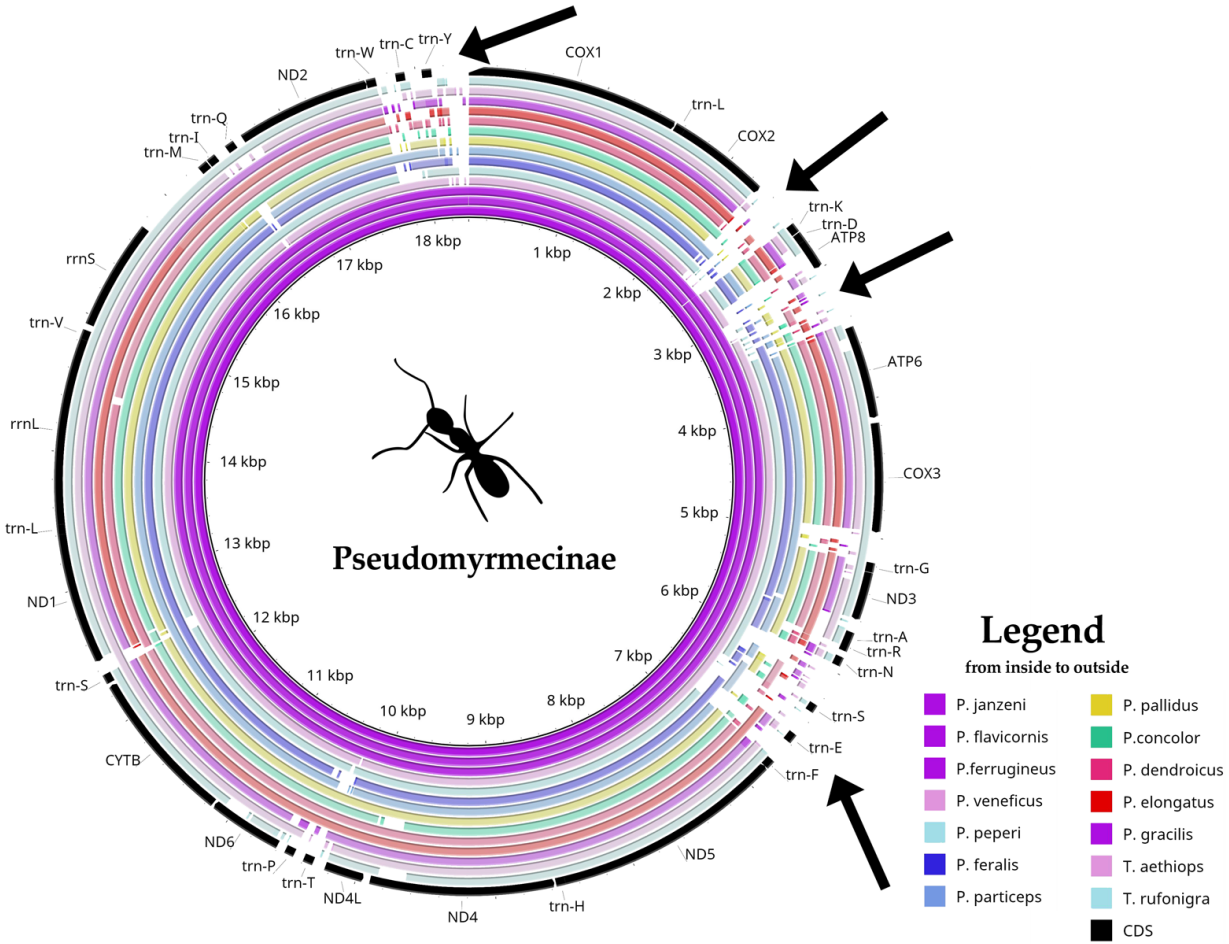
\includegraphics[width=\linewidth]{genomica_comp}
		\caption[Mitogenômica coomparativa de \textit{Pseudomyrmecinae} spp.]{\textbf{Análise de genômica comparativa de todas as 14 formigas da subfamília Pseudomyrmecinae}}
		\legend{Comparação por BLAST de todos os genomas mitocondriais de Pseudomyrmecinae contra uma referência (Pseudomyrmex janzeni) gerada pelo Blast Ring Image Generator (BRIG). As lacunas presentes nos anéis correspondem a regiões com menos de 50 \% de identidade com a seqüência de referência. A maioria das características mitocondriais é conservada dentro do clado, embora ATP8 e alguns tRNAs (trn-S, trn-E e trn-T) tenham apresentado maior variabilidade. Quatro regiões (identificadas por setas) apresentam variações de tamanho de nucleotídeos e são encontradas entre \textbf{(i)} COX2 e trn-K; \textbf{(ii)} ATP8 e ATP6; \textbf{(iii)} trn-N e trn-F e; \textbf{(iv)} trn-W e COX1.}
		\label{fig:genomica_comp}
	\end{figure}
	
	
	\begin{figure}[h]
		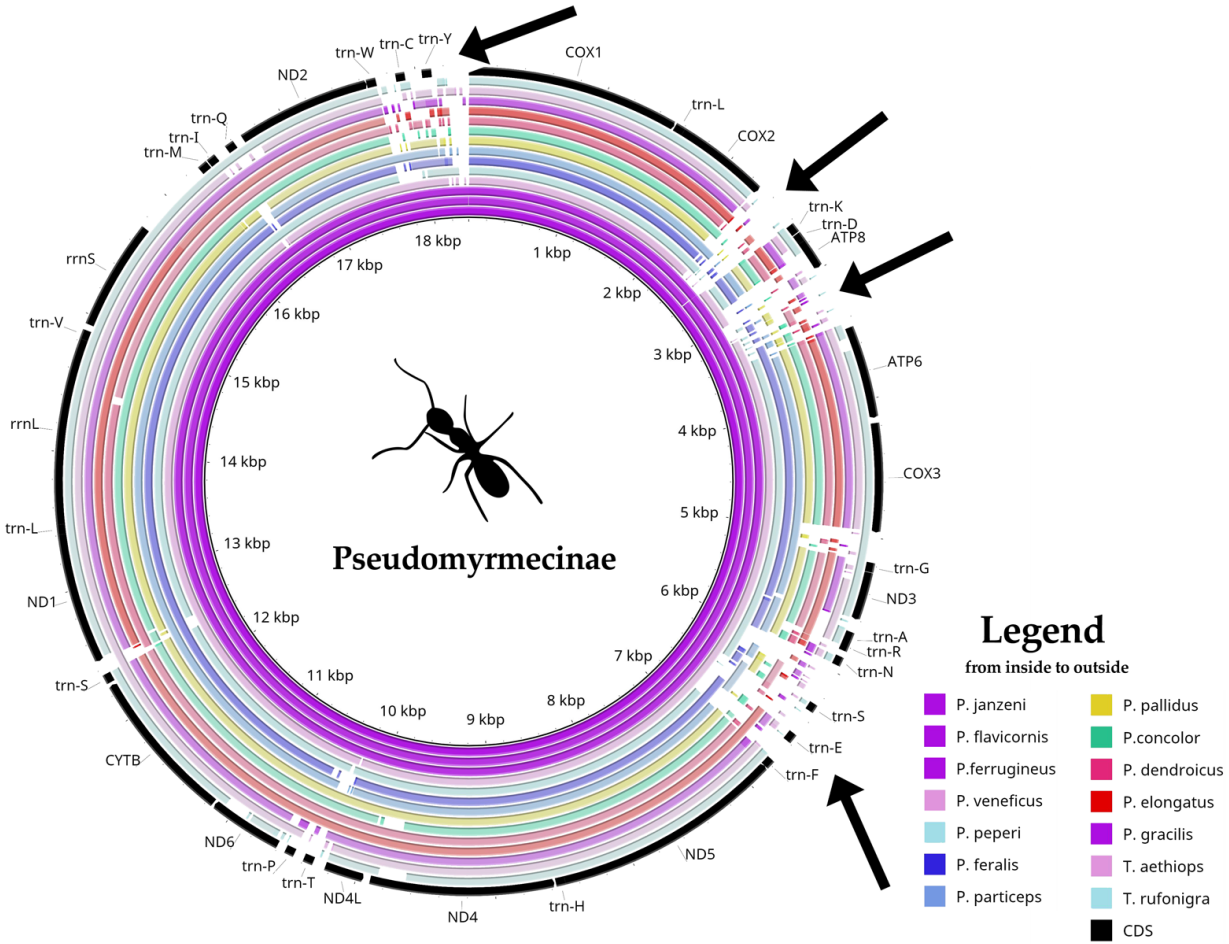
\includegraphics[width=\linewidth]{genomica_comp}
		\caption[Sintenia mitogenômica da família Formicidae]{\textbf{Cinco sintenias observadas em mitogenomas completos da família Formicidae disponíveis no Genbank}}
		\legend{Os dois arranjos gênicos modais estão representados dentro do retângulo horizontal e foram observados em 26 das 29 espécies analizadas: todas as Pseudomyrmecinae (14 espécies); todas as Dolichoderinae (duas espécies: L. pallens e L. humile); três das quatro Formicinae (F. fusca, F. selysi e P. dives) e em sete das nove Myrmicinae (A. texana; C. obscurior; M. scabrinodis; S. richteri; S. geminata; S. invicta; V. emeryi). Nós sugerimos que essas sintenias podem representar arranjos ancestrais para esses clados. As sintenias fora do retângulo horizontal correspondem às ordens gênicas cuja ocorrência é limitada a uma única espécie. Os retângulos verticais e linhas indicam regiões nas quais mudanças de sintenia ocorreram e tanto o asterisco (*) quanto a linha vertical no trn-Y de W. auropunctata indicam que essa é a única feature em uma mitocôndria de formiga que mudou sua fita codificante ao longo de sua evolução.}
		\label{fig:sintenia}
	\end{figure}
	
	

	\section{Análises filogenéticas de Formicidae usando dados mitogenômicos}
	
	Para avaliar a filogenia do grupo, duas árvores de Máxima Verossimilhança foram produzidas usando dados de entrada ligeiramente diferentes: (i) as sequências alinhadas e concatenadas para todos os 13 PCGs mitocondriais (Figura \ref{fig:tree_genes}); e (ii) os genomas mitocondriais completos (Figura \ref{fig:tree_wholemito}). Analisamos todas as espécies de formigas que apresentam mitogenomas completos disponíveis no Genbank (Gotzek et al., 2010; Hasegawa et al., 2011; Berman et al., 2014; Babbucci et al., 2014; Kim et al., 2015; Duan et al., 2016; Liu et al., 2016; Yang et al., 2016) e duas abelhas da família Apidae como outgroups (Crozier \& Crozier, 1993; Cha et al., 2007) (ver números de acesso e referências para todas as sequências na Tabela \ref{tab:s2}. As árvores reconstruídas a partir de dados mitocondriais corroboraram a maioria das relações filogenéticas conhecidas para formigas com vários clados observados como monofiléticos com alta confiança (bootstrap = 100). Ambas as árvores apresentaram resultados semelhantes, embora diferenças possam ser observadas em vários nós quanto à topologia da árvore e/ou suporte estatístico. A principal diferença observada é que a árvore de genes concatenados exibiu todas as subfamílias como monofiléticas, enquanto Myrmicinae foi recuperada como parafilética na árvore baseada em mitogenomas completos. 
	
		\begin{figure}[htb]
		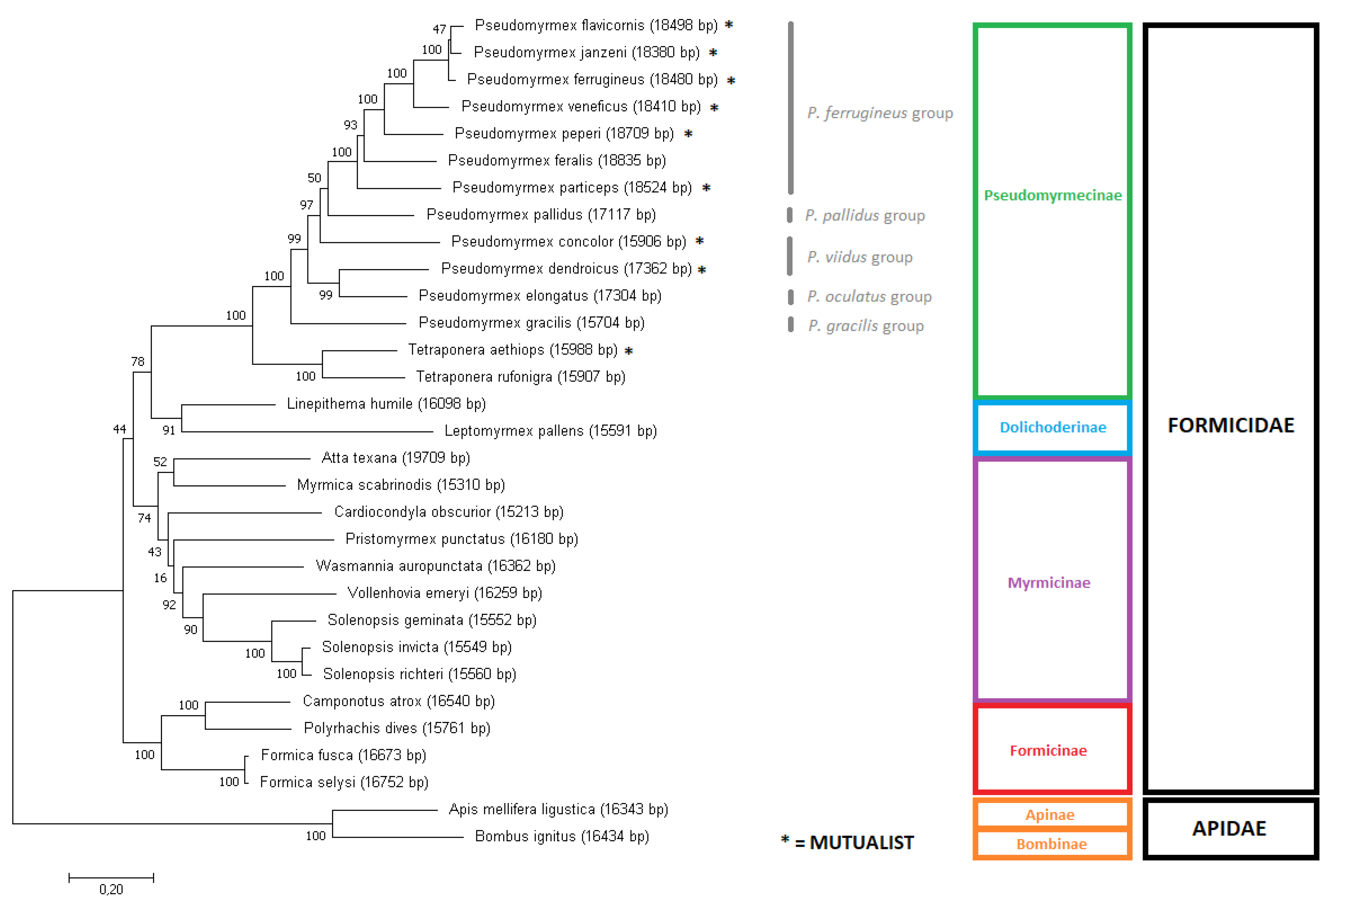
\includegraphics[width=\linewidth]{tree_genes}
		\caption[Árvore de concatenação gênica]{\textbf{Árvore filogenômica de concatenação gênica para todos os mitogenomas completos de Formicidae disponíveis no Genbank}}
		\legend{A árvore foi construída usando as sequências nucleotídicas alinhadas e concatenadas para todos os 13 genes mitocondriais codificadores de proteínas. Modeltest identificou o GTR + G + I como o modelo de substituição mais adequado e a filogenia foi reconstruída por Maximum Likelihood usando o software MEGA7, com 1000 replicatas geradas pelo método de bootstrap. Abelhas da família Apidae foram utilizadas como grupo externo. Grupos de espécies do gênero Pseudomyrmex são evidenciados e espécies de Pseudomyrmecinae que apresentam características mutualistas são indicadas pela presença de um asterisco “*”.}
		\label{fig:tree_genes}
	\end{figure}
	
	\begin{figure}[htb]
		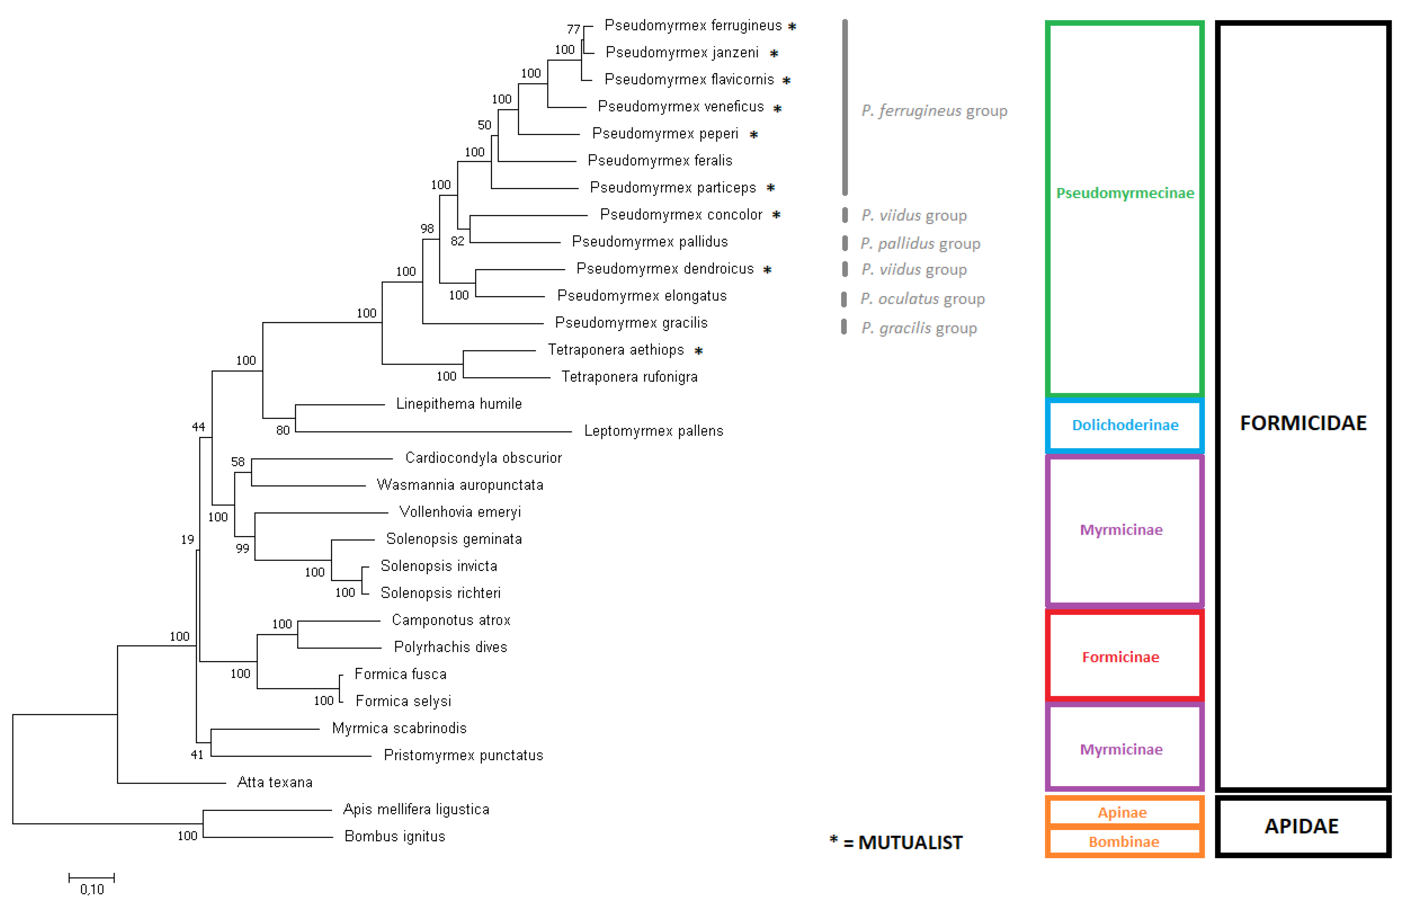
\includegraphics[width=\linewidth]{tree_wholemito}
		\caption[Árvore de sequência mitocondrial completa]{\textbf{Árvore filogenética usando a sequência mitocondrial completa de todos os mitogenomas de formigas disponíveis no Genbank.}}
		\legend{``GTR + G + I'' foi escolhido como modelo de substituição, conforme sugerido pelo software Modeltest. A árvore foi construída usando MEGA7 pelo método de Maximum Likelihood com 1000 replicatas de bootstrap. Mitogenomas de abelhas foram usados como grupos externos. Grupos de espécies de Pseudomyrmex e espécies mutualistas de Pseudomyrmecinae são evidenciados.}
		\label{fig:tree_wholemito}
	\end{figure}
	
\end{document}